% \section{Κομμένα}

\graphicspath{{Chapter2/Figs/Vector/}{Chapter2/Figs/Raster/}{Chapter3/Figs/Vector/}{Chapter4/Figs/Vector/}{Chapter5/Figs/Vector/}{Chapter6/Figs/Vector1/}{Chapter7/Figs/Vector/}{Chapter8/Figs/Vector/}}

% ----------------------------------------------------------------------------
% % CHAPTER 2
%-----------------------------------------------------------------------------

\begin{frame}
  \frametitle{Πρόσφατες εργασίες για την περιοχή}
  \label{fr2:previousIonio}
\begin{columns}
  \begin{column}{.49\textwidth}
  \begin{block}{\textcite{Chousianitis2015}}
  \begin{footnotesize}
    Βόρειo Ιόνιο: Επιμήκυνση Β-Ν.\\
    Κεντρικό: Περιστροφική Κίνηση 6-8$^{\circ}$/My.\\
    Νότιο: Επιμήκυνση ΔΝΔ-ΑΒΑ.\\
    Κορινθιακός: Επιμήκυνση Β-Ν.
  \end{footnotesize}
  \end{block}
  \centering
    \includegraphics[width=.8\linewidth]{chousian2015.png}
%     {\tiny \parencite{Chousianitis2015}}
  \end{column}
  \begin{column}{.49\textwidth}
  \begin{block}{\textcite{Perouse2013}}
\begin{footnotesize}
  Κεντρικό Ιόνιο ως ξεχωριστό μπλοκ.\\
  Διερεύνηση των ορίων στη Δυτική πλευρά.
  \end{footnotesize}
  \end{block}
  \centering
    \includegraphics[width=.8\linewidth]{perouseZones344.png}
%     {\tiny \parencite{Perouse2013}}
  \end{column}
\end{columns}

\end{frame}
\note{}


\begin{frame}
  \frametitle{Υπάρχουσες εργασίες}
  \framesubtitle{Σεισμολογικά Δεδομένα}
  \label{fr2:pr_seism}
    \begin{block}{\textcite{Papazachos1971}}%<1->
    Ερμηνεία των τεκτονικών και γεωφυσικών χαρακτηριστικών του Ελληνικού τόξου.
    \end{block}
    \begin{block}{\textcite{McKenzie1972}}%<2->
    Προτείνονται 2 μικροπλάκες, του Νοτίου Αιγαίου και της Κεντρικής-Βορείου Ελλάδος.
    \end{block}
    \begin{block}{\textcite{LePichon1979}}%<3>
    Επιλύσεις των μηχανισμών γένεσης για την εκτίμηση του πεδίου παραμόρφωσης της Ανατολικής
    Μεσογείου.
    \end{block}
    % \footfullcite{Papazachos1971}
    % \footfullcite{Drewes1982}
\end{frame}
\note{}

\begin{frame}
  \frametitle{Υπάρχουσες εργασίες}
  \framesubtitle{Γεωδαιτικά Δεδομένα}
  \label{fr2:pr_geod}
    \begin{block}{\textcite{Drewes1982}}
    Δεδομένα 20 γεωδαιτικών σταθμών παρατήρησης με την τεχνική SLR.\par
    Εκτίμηση της περιστροφικής κίνησης των δύο μικροπλακών στην Ανατολική Μεσόγειο
    \end{block}
\vskip-.2cm
    \begin{block}{\textcite{Billiris1991}}
    Μετρήσεις του τριγωνομετρικού δικτύου 1\textsuperscript{ης} τάξης των περιόδων 1890, 1980.\par
    Σχετική μετατόπιση στον Κορινθιακό Κόλπο από 40 έως 60 cm.\par
    Νοτιοδυτική κίνηση της Πελοποννήσου σε σχέση με τη Βόρεια Ελλάδα.
    \end{block}
\vskip-.2cm
    \begin{block}{\textcite{stiros1993283}}
    38 τριγωνομετρικά σημεία στην Κεντρική Ελλάδα, κοινά σε τρεις διαφορετικές περιόδους\par
    Aριστερόστροφη διάτμηση και διαστολή σε διεύθυνση Β - Ν στον Κορινθιακό Κόλπο μετά το 1930
    \end{block}
\end{frame}
\note{}

\begin{frame}
  \frametitle{Υπάρχουσες εργασίες}
  \framesubtitle{Γεωδαιτικά Δεδομένα}
  \label{fr2:pr_geod2}
\begin{columns}
  \begin{column}{.49\textwidth}
    \begin{block}{\textcite{Veis1992}}
    75 κοινά σημεία των τριγωνισμών \par περιόδων 1890-1982.\par
    Η περιοχή μελέτης διαιρέθηκε σε 9 μπλοκ ομοιογενούς παραμόρφωσης.
    \end{block}
    
    \begin{block}{\textcite{Davies199724571}}
    36 σημεία, επαναμέτρηση με GPS, το 1992.\par
    Σταθμοί SLR Διόνυσος \& Χρυσοκελλαριά\par
    Μετρήσεις σε 10 έκκεντρα.
    \end{block}
  \end{column}
  \begin{column}{.49\textwidth}
  \centering
    \includegraphics[width=.7\linewidth]{veis92_9bl.jpg}

    \includegraphics[width=.7\linewidth]{davies97_tr.png}

  \end{column}
\end{columns}
\end{frame}
\note{}

\begin{frame}
  \frametitle{Υπάρχουσες εργασίες}
  \framesubtitle{Γεωδαιτικά Δορυφορικά Δεδομένα}
  \label{fr2:pr_satgeod2}
  \vskip-.2cm
\begin{columns}[t]
  \begin{column}{.48\textwidth}
    \begin{block}{\textcite{Nyst2004}}
    375 σταθμοί GPS\par
    4 μικροπλάκες\par
%     \begin{itemize}
%       \item Κεντρική Ελλάδα\\
%       \item Νότιο-Κεντρικό Αιγαίο\\
%       \item Ανατολία\\
%       \item Νότιος Μαρμαράς\\
%     \end{itemize}
    \end{block}
    \centering
    \includegraphics[width=.91\linewidth]{nyst04_4bl.png}
  \end{column}
  \begin{column}{.48\textwidth}
    
\begin{block}{\textcite{Reilinger2006}}
440 σταθμοί GPS\par
8 μικροπλάκες
\end{block}
    \centering
    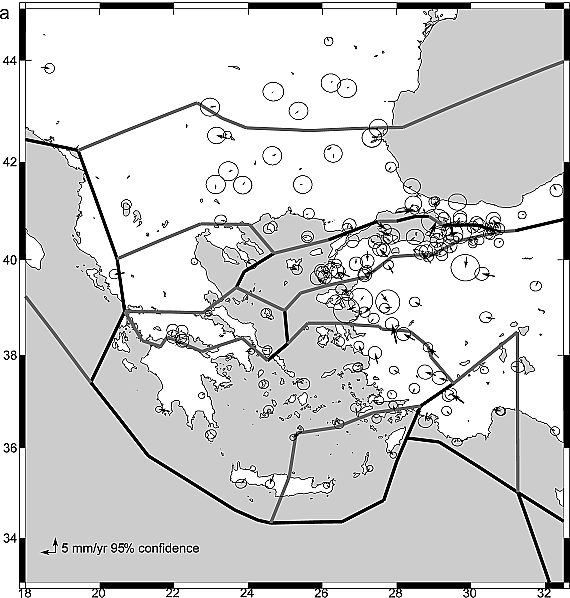
\includegraphics[width=.84\linewidth]{reilinger06_8bl.png}
  \end{column}
\end{columns}
\end{frame}
\note{}

\begin{frame}
  \frametitle{Υπάρχουσες εργασίες}
  \framesubtitle{Γεωδαιτικά Δορυφορικά Δεδομένα}
  \label{fr2:satgeod3}
\begin{columns}
  \begin{column}{.48\textwidth}
    \begin{block}{\textcite{Taymaz1991,Floyd2010}}
    254 σταθμοί GPS\par
    10 μικρομπλόκ
    \end{block}
    \centering  
    \includegraphics[width=.92\linewidth]{floyd10_10bl.png}
  \end{column}
  \begin{column}{.48\textwidth}
    \begin{block}{\textcite{Floyd2010}}
    254 σταθμοί GPS\par
    15 μικρομπλόκ
    \end{block}
    \vskip .4cm
    \centering  
    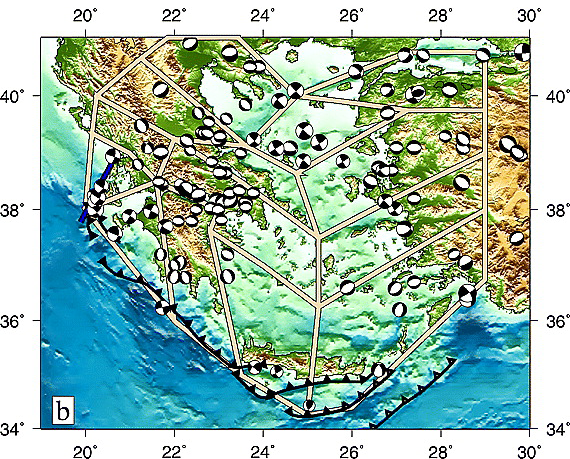
\includegraphics[width=.92\linewidth]{floyd10_15bl.png}
  \end{column}
\end{columns}
% \footfullcite{Floyd2010}
\end{frame}
\note{}



% ----------------------------------------------------------------------------
% % CHAPTER 3
%-----------------------------------------------------------------------------
\begin{frame}
  \frametitle{Αλγόριθμος Frank}
  \framesubtitle{}
  \label{fr3:frank}
  Προϋποθέτει επαναλαμβανόμενες μετρήσεις που έχουν πραγματοποιηθεί στις κορυφές ενός τριγωνομετρικού δικτύου οριζόντιου ελέγχου.
  \begin{equation*}
  \label{eq:velgrad22}
    E=\begin{bmatrix}
    \varepsilon_{11} & \varepsilon_{12}\\ 
    \varepsilon_{21} & \varepsilon_{22}
    \end{bmatrix}
  \end{equation*}
  
  Οι διατμητικές συνιστώσες της ανηγμένης παραμόρφωσης και η περιστροφή:\\
  \[    \gamma _1=\varepsilon_{11} - \varepsilon_{22}, 
  \hspace{.7cm}
      \gamma _2=\varepsilon_{12} + \varepsilon_{21}, 
  \hspace{.7cm}
      \omega = \frac{1}{2} \left (\varepsilon_{12} - \varepsilon_{21}  \right )\]
  
  Η τιμή της ολικής διάτμησης και το αζιμούθιο των κύριων αξόνων της έλλειψης της ανηγμένης παραμόρφωσης:
  \[ \gamma = \sqrt{{\gamma_{1}}^{2}+{\gamma_{2}}^{2}}
  \hspace{1cm}
  \tan 2\psi = \frac{\gamma_1}{\gamma_2} \]


\end{frame}
\note{}

\begin{frame}
  \frametitle{Αλγόριθμος Frank}
  \framesubtitle{Ανάλυση στο τρίγωνο}
  \label{fr3:frank_tr}
  \begin{columns}
    \begin{column}{.65\textwidth}
      Η διαφορά της γωνίας σε δύο χρονικές στιγμές:
      \[ \delta\phi_\alpha=\delta \theta_\beta - \delta \theta_\gamma \]
      
      Θεωρείται ότι η παραμόρφωση είναι ομοιόμορφη σε όλη τη περιοχή του τριγώνου.
      \begin{scriptsize}
      \begin{align*}
\delta\phi_\alpha = \frac{1}{2}\left ( \sin2\theta_\beta - \sin2\theta_\gamma \right )\gamma_1 + \left ( \cos2\theta_\beta - \cos2\theta_\gamma \right )\gamma_2 \\
\delta\phi_\beta = \frac{1}{2}\left ( \sin2\theta_\gamma - \sin2\theta_\alpha \right )\gamma_1 + \left ( \cos2\theta_\gamma -\cos2\theta_\alpha \right )\gamma_2
\end{align*}
      \end{scriptsize}

    \end{column}
    \begin{column}{.34\textwidth}
      \centering
          \adjincludegraphics[width=.98\linewidth, valign=t]{FrankTR.jpg}
          
          {\tiny \parencite{Frank1966}}
    \end{column}
  \end{columns}

  \begin{footnotesize}
  \begin{align*}
  \gamma_1=\frac{\sin\left ( \theta_\gamma + \theta_\alpha \right )\left ( \delta\phi_\alpha/\sin\alpha_\alpha \right ) - \sin\left ( \theta_\beta + \theta_\gamma \right )\left ( \delta\phi_\beta/\sin\alpha_\beta \right )}{\sin\phi_\gamma} \\
  \gamma_2=\frac{\cos\left ( \theta_\gamma + \theta_\alpha \right )\left ( \delta\phi_\alpha/\sin\alpha_\alpha \right ) - \cos\left ( \theta_\beta + \theta_\gamma \right )\left ( \delta\phi_\beta/\sin\alpha_\beta \right )}{\sin\phi_\gamma}
  \end{align*}
  \end{footnotesize}

\end{frame}
\note{}

% ----------------------------------------------------------------------------
% % CHAPTER 4
%-----------------------------------------------------------------------------


% ----------------------------------------------------------------------------
% % CHAPTER 5
%-----------------------------------------------------------------------------
\begin{frame}
  \frametitle{Διαχρονική Ανάλυση}
  \framesubtitle{Η περιοχή της Δυτικής Ελλάδας}
  \label{fr5:allpp_ionio}
  \begin{columns}
    \begin{column}{.5\textwidth}
    \centering
      \textcolor{red}{\small Άξονες επιμήκυνσης}\\
      \includegraphics[width=\linewidth]{ext_ionio.jpg}

    \end{column}
    \begin{column}{.5\textwidth}
    \centering
      \textcolor{blue}{\small Ολική διάτμηση ($\dot{\gamma}_{tot}$)}\\
      \includegraphics[width=\linewidth]{shear_ionio.jpg}

    \end{column}
  \end{columns}
\end{frame}
\note{}


% ----------------------------------------------------------------------------
% % CHAPTER 6
%-----------------------------------------------------------------------------
\begin{frame}
  \frametitle{Επίγεια \& Δορυφορικά Γεωδαιτικά Δεδομένα}
  \framesubtitle{}
  \label{fr6:terr_sat_ext}
  \begin{columns}
    \begin{column}{.5\textwidth}
     \centering
     {\footnotesize  Άξονες επιμήκυνσης,\\ επίγειες παρατηρήσεις}\\
      \includegraphics[width=.9\linewidth]{ext_ionio.jpg}

    \end{column}
    \begin{column}{.5\textwidth}
    \centering
    {\footnotesize  Κύριοι άξονες ($\dot{e}_{max}$, $\dot{e}_{min}$).}\\
      \includegraphics[width=\linewidth]{ciontrSTR.jpg}

    \end{column}
  \end{columns}
\end{frame}
\note{}

\begin{frame}
  \frametitle{Περιοχή Κεντρικού Ιονίου -Πατραϊκού Κόλπου}
  \framesubtitle{Μοντέλο 5 μπλοκς}
  \label{fr6:str_5bl}
  \vskip.1cm
  \begin{columns}
    \begin{column}{.5\textwidth}
    \centering
    {\footnotesize  Κύριοι άξονες ($\dot{e}_{max}$, $\dot{e}_{min}$).}\\
      \includegraphics[width=\linewidth]{ptr05bSTR.jpg}

    \end{column}
    \begin{column}{.5\textwidth}
    \centering
      {\footnotesize  Ρυθμός περιστροφής ($\dot{\Omega}$).}\\
      \includegraphics[width=\linewidth]{ptr05bROT.jpg}

    \end{column}
  \end{columns}
  \vskip-.1cm
  \begin{table}[H]{\tiny
     \begin{center}
      \begin{tabular*}{\linewidth}{@{\extracolsep{\fill}}c c c c c c}
\toprule
% \multicolumn{1}{r}{} &\multicolumn{5}{c}{blocks} \\
% \cline{2-6}
\multicolumn{1}{r}{} &1 & 2 & 3 & 4 & 5\\
\midrule
%  φ  & 38.185 & 38.607 & 38.317 & 37.907 & 38.385 \\
%  λ  & 21.019 & 21.726 & 21.996 & 21.731 & 21.617 \\
 $\dot{e}_{max}$ $\pm$ σ$_{\dot{e}_{max}}$  &  +0.058 $\pm$ 0.027 & +0.050 $\pm$ 0.051 & +0.411 $\pm$ 0.083 & +0.011 $\pm$ 0.045 & +0.293 $\pm$ 0.073 \\
 $\dot{e}_{min}$ $\pm$ σ$_{\dot{e}_{min}}$  &  -0.104 $\pm$ 0.029 & -0.032 $\pm$ 0.038 & -0.098 $\pm$ 0.112 & -0.050 $\pm$ 0.050 & -0.087 $\pm$  0.089\\
 Az$_{\dot{e}_{max}}$ $\pm$ σ$_{Az_{\dot{e}_{max}}}$ & -11.185 $\pm$  6.041 & 25.962 $\pm$ 23.816 & 13.949  $\pm$  6.932 & 16.187 $\pm$ 28.914 & 12.255 $\pm$  7.544\\
 $\dot{\Omega}$  $\pm$ σ$_{\dot{\Omega}}$ & +7.439 $\pm$ 0.973 & +3.605 $\pm$  1.946 & -0.401 $\pm$ 3.548 & +2.976 $\pm$ 1.774 & +6.294 $\pm$  2.861 \\
 $\dot{\gamma}_{tot}$ $\pm$ σ$_{\dot{\gamma}_{tot}}$ & 0.162 $\pm$ 0.040 & 0.082 $\pm$ 0.064 & 0.509 $\pm$ 0.140 & 0.061 $\pm$ 0.068 & 0.380 $\pm$  0.115 \\
\bottomrule
\multicolumn{6}{l}{φ, λ, Az$_{\dot{e}_{max}}$ in deg; $\dot{e}_{max}$, $\dot{e}_{min}$, $\dot{\gamma}_{tot}$ in μstrain/y ;  $\dot{\Omega}$ in deg/My }
   \end{tabular*}
 \end{center}}
\end{table}
\end{frame}
\note{}


% ----------------------------------------------------------------------------
% % CHAPTER 7
%-----------------------------------------------------------------------------


% ----------------------------------------------------------------------------
% % CHAPTER 8
%-----------------------------------------------------------------------------

\begin{frame}
  \frametitle{Συμπεράσματα}
  \framesubtitle{Εκτίμηση επιφανειακών παραμορφώσεων}
  \label{fr8:concl2}
  \begin{itemize}
    \item 1η π.α.: Ολική διάτμηση της τάξης των 80 nstrain/y.\\
    \item 2η - 3η π.α.: Αύξηση των τιμών ολικής διάτμησης.\\
%     \item Διαφορές στο πεδίο παραμόρφωσης πριν και μετά το 1930 στον σε Πατραϊκό Κορινθιακό Κόλπο.\\
  \end{itemize}
  \textbf{Δυτική Ελλάδα:}
  \begin{itemize}
    \item Αλλαγή στο πεδίο παραμόρφωσης πριν και μετά το 1930.\\
    \item Πατραϊκός-Κορινθιακός: Αλλαγή στη διεύθυνση της ολικής διάτμησης σε ΑΝΑ - ΔΒΔ, παράλληλα στη διεύθυνση των ρηγμάτων.\\
    \item Επιμήκυνση της περιοχής σε διεύθυνση Β - Ν.\\
  \end{itemize}
  \textbf{Ανατολική Στερεά:}
  \begin{itemize}
    \item Επανιδρύθηκαν πολλά τριγωνομετρικά σημεία.\\
    \item Επιμήκυνση της περιοχής στη διεύθυνση ΒΑ - ΝΔ \parencite{Veis1992,Davies199724571}.\\
    \item 3η π.α, Καπαρέλλι-Ερυθρές: Επιμήκυνση ΒΒΔ - ΝΝΑ.\\
    Δεν συμφωνεί με τη γενική κινηματική εικόνα της περιοχής, συμφωνεί με \textcite{Marinou2015a}. \\
  \end{itemize}
\end{frame}
\note{}









